%% LyX 2.1.3 created this file.  For more info, see http://www.lyx.org/.
%% Do not edit unless you really know what you are doing.
\documentclass[oneside,english]{amsart}
\usepackage[]{fontenc}
\usepackage{amsthm}
\usepackage{graphicx}

\makeatletter
%%%%%%%%%%%%%%%%%%%%%%%%%%%%%% Textclass specific LaTeX commands.
\numberwithin{equation}{section}
\numberwithin{figure}{section}

\makeatother

\usepackage{babel}
\begin{document}

\title{Finance}


\author{Michael Peters}


\thanks{\today{}}

\maketitle
The edgeworth box provides a nice way to think about trade in markets.
The kind of market for which that theory probably best applies is
financial markets. This note explains how to use the edgeworth box
to understand asset pricing.

The approach begins with two traders and two goods. The first step
to understanding all this is to think about income in different states
as representing two distinct goods. Insurance is an example in which
this is true. An insurance policy only pays you money if you have
an accident. Money means a lot more to you when you have an accident
than when you don't, which is why you might be willing to give up
money when you don't have an accident by paying an insurance premium
in order to get it when you do have an accident.

Lets start with a simple Walrasian equilibrium in a two good exchange
economy similar described with an Edgeworth box.

\begin{center}
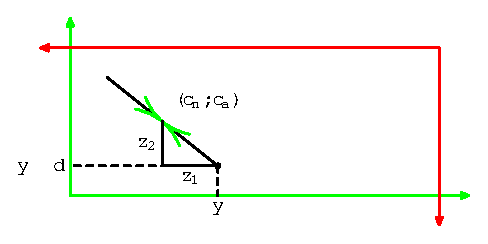
\includegraphics{/home/peters/files/docs/book/finance/finance_fig1}
\par\end{center}

The figure describes a Walrasian equilibrium for an economy with two
goods. Trader 1 starts at the origin, and has quantity $y$ of good
1 and $y-d$ of good 2. He makes a trade with trader to in which he
exchanges $z_{1}$ units of good 1 for $z_{2}$ units of good 2. This
takes both of them to the point where the indifference curves are
tangent so that the allocation is pareto optimal.

In finance, we want to interpret the goods by imagining that there
is an as yet unrealized event, say a recession. Trader 1 has income
$y$ if there is no recession, but has much lower income $y-d$ if
there is.

Before it is known whether or not the recession occurs, there is a
market in which two 'securities' can be traded. The first security,
$a$, pays $1$ dollar if and only if there is no recession. Security
$b$ pays $1$ dollar if and only if there \emph{is }a recession.
We imagine that the way the event contingent transfer occurs is that
trader 1 sells $z_{1}$ unit of security $a$, for which he receives
total revenue $qz_{1}$. He uses the revenue to buy $z_{2}=qz_{1}$
units of security $b$ from individual 2.

The, once the event is realized, when a recession occurs, trader 2,
since she has sold $z_{2}$ units of security $b$, is obliged to
pay $1$ $z_{2}$ dollars. If the recession doesn't occur, then $1$
is on the hook since he is the one who sold off $z_{1}$units of security
$a$.

There is a second way to look at this tradeoff. From $1$'s perspective,
what he does is to plan how much income he would like to have in each
of the two events. His plan is to arrange it so that he has income
$c_{n}$ if there is no recession and $c_{a}$ when there is a recession.
To accomplish this, he realizes that he has to purchase and sell assets
that will force him to pay $z_{1}$ if there is no recession, but
will leave him with a payment of $z_{2}$ when a recession occurs.

The way he might do this is to take the matrix of asset returns, given
by 
\[
\left[\begin{array}{cc}
1 & 0\\
0 & 1
\end{array}\right]
\]
 and post multiply it by his portfolio $\left(z_{1},z_{2}\right)$
viewed as a column vector to get the payments that he wants. In other
words, he would solve the equation
\[
\left[\begin{array}{c}
c_{n}-y\\
c_{a}-y+d
\end{array}\right]=\left[\begin{array}{cc}
1 & 0\\
0 & 1
\end{array}\right]\cdot\left[\begin{array}{c}
z_{1}\\
z_{2}
\end{array}\right]
\]
 which obviously has the solution described above.

As we are working here with a Walrasian equilibrium, trader 2 is happy
with the trade she makes, which is to receive $c_{n}-y$ when there
is no recession, but to pay $c_{a}-y+d$ when there is.

At this point, we could ask what the prices of the securities have
to be so that the market for them clears. To see this, we just consider
the Walrasian equilibrium first and imagine that the price of good
1 is $q$ while the price of good 2 is $1.$ The bundle $\left(c_{n},c_{a}\right)$
has cost $qc_{n}+c_{a}$which is equal to $qy+y-d$ since it is a
Walrasian equilibrium. Then of course, $q\left(c_{n}-y\right)+\left(c_{a}-y+d\right)=0$,
from which it is obvious that the price of asset $a$ has to be $q$
to get this to work.

We could express this as a problem is computing a security price $\rho$
for asset 1 such that
\[
\rho z_{1}+z_{2}=\rho\left(c_{n}-y\right)+\left(c_{a}-y+d\right)=0
\]
or
\[
\rho=-\frac{c_{a}-y+d}{c_{n}-y}=q.
\]


So far this is pretty obvious, so lets enrich the model to make it
look more like a stock market. Suppose that our two traders are entrepreneurs.
Each of them has an inheritance $\omega$ that they have no matter
what. But each has a start up venture they are running. The start
up of trader 1 gives profits $\pi_{a1}>0$ if there is no recession
and $\pi_{a2}<0$ if there is. Trader 2 has another start up that
does well in a recession. Her company earns $\pi_{b1}<0$ if there
is no recession, but make a profit $\pi_{b2}$ if there is a recession.

Now lets take the first figure above, and just relabel it so that
it coincides with this new information.

\begin{center}
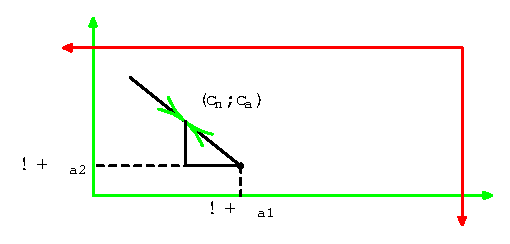
\includegraphics{/home/peters/files/docs/book/finance/finance_fig2}
\par\end{center}

Here is the same diagram with the trades labeled.

\begin{center}
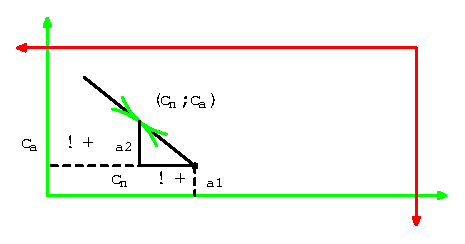
\includegraphics{/home/peters/files/docs/book/finance/finance_fig3}
\par\end{center}

Now we can imitate what we did before. We'll let $q=\frac{c_{a}-\omega-\pi_{a2}}{c_{n}-\omega-\pi_{a1}}$
be the price ratio that seems to support the Walrasian equilibrium.

To support this outcome, trader 1 has to buy a portfolio $\left(z_{1},z_{2}\right).$
As the assets are now profits in start up companies, the portfolio
has to satisfy the following matrix equation:
\[
\left[\begin{array}{c}
c_{n}-\omega-\pi_{a1}\\
c_{a}-\omega-\pi_{a2}
\end{array}\right]=\left[\begin{array}{cc}
\pi_{a_{1}} & \pi_{b1}\\
\pi_{a2} & \pi_{b_{2}}
\end{array}\right]\cdot\left[\begin{array}{c}
z_{1}\\
z_{2}
\end{array}\right]
\]
It is straightforward how we should do this, pre multiply both sides
of the equation by the inverse matrix
\[
\left[\begin{array}{cc}
\pi_{a_{1}} & \pi_{b1}\\
\pi_{a2} & \pi_{b_{2}}
\end{array}\right]^{-1}\left[\begin{array}{c}
c_{n}-\omega-\pi_{a1}\\
c_{a}-\omega-\pi_{a2}
\end{array}\right]=
\]
\[
\frac{1}{\pi_{a1}\pi_{b2}-\pi_{b1}\pi_{a_{2}}}\left[\begin{array}{cc}
\pi_{b2} & -\pi_{b1}\\
-\pi_{a2} & \pi_{a_{1}}
\end{array}\right]\left[\begin{array}{c}
c_{n}-\omega-\pi_{a1}\\
c_{a}-\omega-\pi_{a2}
\end{array}\right]=\left[\begin{array}{c}
z_{1}\\
z_{2}
\end{array}\right]
\]
 So we can compute the portfolio rather easily. The interpretation
is just as before. Trader 1 is going to sell off $z_{1}$ of the shares
in his venture and use the proceeds to purchase shares in the venture
being run by trader 2.

All we have left to do at this point is to try to figure out how the
shares of the two ventures should be priced. Lets use the convention
that the shares in venture 2 should have a price 1, so that all we
need to figure out is what the corresponding relative price $\rho$
should be of the shares in venture 1.

Now it is just computation. We have to have $\rho z_{1}+z_{2}=0$,
which means
\[
\frac{1}{\pi_{a1}\pi_{b2}-\pi_{b1}\pi_{a_{2}}}\left[\begin{array}{cc}
\rho & 1\end{array}\right]\left[\begin{array}{cc}
\pi_{b2} & -\pi_{b1}\\
-\pi_{a2} & \pi_{a_{1}}
\end{array}\right]\left[\begin{array}{c}
c_{n}-\omega-\pi_{a1}\\
c_{a}-\omega-\pi_{a2}
\end{array}\right]=0
\]
If we want to solve this, we can obviously forget about the constant
$\frac{1}{\pi_{a1}\pi_{b2}-\pi_{b1}\pi_{a_{2}}}$ and solve
\[
\left[\begin{array}{cc}
\rho & 1\end{array}\right]\left[\begin{array}{cc}
\pi_{b2} & -\pi_{b1}\\
-\pi_{a2} & \pi_{a_{1}}
\end{array}\right]\left[\begin{array}{c}
c_{n}-\omega-\pi_{a1}\\
c_{a}-\omega-\pi_{a2}
\end{array}\right]=0
\]
instead. This gives first
\[
\left[\begin{array}{cc}
\rho\pi_{b2}-\pi_{a2} & \pi_{a1}-\rho\pi_{b1}\end{array}\right]\left[\begin{array}{c}
c_{n}-\omega-\pi_{a1}\\
c_{a}-\omega-\pi_{a2}
\end{array}\right]=0
\]
or
\[
\left(\rho\pi_{b2}-\pi_{a2}\right)\left(c_{n}-\omega-\pi_{a1}\right)+\left(\pi_{a1}-\rho\pi_{b1}\right)\left(c_{a}-\omega-\pi_{a2}\right)=0.
\]
From the Walrasian equilibrium, this is
\[
\left(\rho\pi_{b2}-\pi_{a2}\right)=-q\left(\pi_{a1}-\rho\pi_{b1}\right)
\]
or
\[
\rho=-\frac{q\pi_{a1}-\pi_{a_{2}}}{\pi_{b2}-q\pi_{b1}}.
\]


So this formula describes the basics of asset pricing. To compute
the value of an asset, you need to know a couple of things. The first
of which is the returns on other assets - even though we are trying
to find the relative price of asset $a$ we have to know $\pi_{b1}$
and $\pi_{b2}$ to do that. Second, we need to know the state price
$q$, which we can compute by solving for a Walrasian equilibrium.
\end{document}
